\documentclass{boi2014-lt}

\usepackage{enumitem}

\renewcommand{\DayNum}{2}
\renewcommand{\TaskCode}{postmen}
\renewcommand{\TaskName}{Paštininkai senjorai}

\begin{document}
    \begin{wrapfigure}[8]{r}{4cm}
        \vspace{-18pt}
        \includegraphics[width=4cm]{\TaskCode.jpeg}
    \end{wrapfigure}
    Dabar 2036-ieji metai ir Europa yra perpildyta garbaus amžiaus piliečiais.
    Tam, kad jie išliktų sveiki, Europos daugumų ministerija (garbaus amžiaus
    piliečiai \emph{yra} dauguma!) siūlo įdarbinti juos popierinių laiškų,
    kurie vis dar yra siunčiami (dažniausiai būtent garbaus amžiaus piliečiams),
    išnešiotojais. Šis pasiūlymas bus realizuotas visoje Europoje.

    Ministerija sukūrė „garbaus amžiaus paštininkų sistemą“ padalindama visą
    Europą į pašto rajonus. Pašto rajonas -- tai gatvių tinklas, sudarytas iš
    gatvių ir sankryžų. Kiekviena gatve šiame tinkle galima eiti abejomis
    kryptimis. Kiekviename rajone paštininkais galima pasamdyti neribotą skaičių
    garbaus amžiaus piliečių. Kiekvieną rytą, kiekvienas paštininkas gauna krepšį
    su laiškais, kuriuos reikia pristatyti keliaujant maršrutu, dengiančiu dalį
    gatvių tinklo. Kiekvienas maršrutas turi būti tinkamas garbiam amžiui, t.~y.
    jis turi tenkinti šias sąlygas:
    \begin{itemize}
        \item Prasidėti ir baigtis toje pačioje sankryžoje.
        \item Nekirsti jokios sankryžos daugiau nei vieną kartą. (Nepainiokite
            garbaus amžiaus piliečių.)
        \item Neturėti bendrų gatvių su kitais maršrutais, t.~y. kiekvieną gatvę
            aptarnauja lygiai vienas paštininkas. (Garbaus amžiaus piliečiai
            neturėtų peštis tarpusavyje.)
    \end{itemize}

    Visi maršrutai kartu privalo pilnai padengti duotą gatvių tinklą: t.~y.
    kiekviena tinklo gatvė turi būti lygiai vieno maršruto dalimi.

    \Task
    Ministerija prašo jūsų sukurti programą, kuri duotam pašto rajono gatvių
    tinklui surastų garbiam amžiui tinkamų maršrutų aibę, kuri pilnai padengtų
    gatvių tinklą.

    \Input
    Įvestis apibūdina gatvių tinklą.
    
    Pirmoje eilutėje yra du sveikieji skaičiai $N$ ir $M$ -- atitinkamai
    sankryžų skaičius ir gatvių skaičius. Sankryžos numeruojamos nuo $1$ iki $N$.

    Toliau kiekvienoje iš $M$ eilučių yra du sveikieji skaičiai $u$ ir $v$
    ($1 \le u, v \le N, u \neq v$), reiškiantys, kad sankryžas Nr. $u$ ir Nr.
    $v$ jungia gatvė.

    Kiekvienai įvesčiai galioja:
    \begin{enumerate}
        \item Kiekvieną sankryžų porą jungia ne daugiau nei viena gatvė.
        \item Iš bet kurios sankryžos galima pasiekti bet kurią kitą keliaujant
            viena arba daugiau gatvių.
        \item Sprendinys visada egzistuoja, t.~y. visada galima rasti garbiam
            amžiui tinkamų maršrutų aibę, kuri pilnai padengia gatvių tinklą.
    \end{enumerate}

    \Output
    
    Kiekviena eilutė turi atitikti vieną garbiam amžiui tinkamą maršrutą --
    joje turi būti išvardytos maršrutą sudarančios sankryžos ta tvarka, kuria
    jas aplanko paštininkas. Pradinę ir galinę sankryžą išveskite pirmą (ir ją
    išveskite tik kartą).

    Jeigu egzistuoja keletas sprendinių, jūsų programa gali išvesti bet kurį
    iš jų.

    \Example

    \example
    {
        10 15 \newline
        1 3 \newline
        5 1\newline
        2 3 \newline
        9 2\newline
        3 4 \newline
        6 3\newline
        4 5 \newline
        7 4\newline
        4 8 \newline
        5 7 \newline
        8 5\newline
        6 7 \newline
        7 8 \newline
        8 10 \newline
        10 9
    }
    {
        2 3 4 5 8 10 9 \newline
        7 8 4\newline
        1 5 7 6 3
    }
    {
        Pateiktas paveikslėlis iliustruoja gatvių tinklą ir tris garbiam amžiui
        tinkamus maršrutus, kurie pilnai jį padengia.

        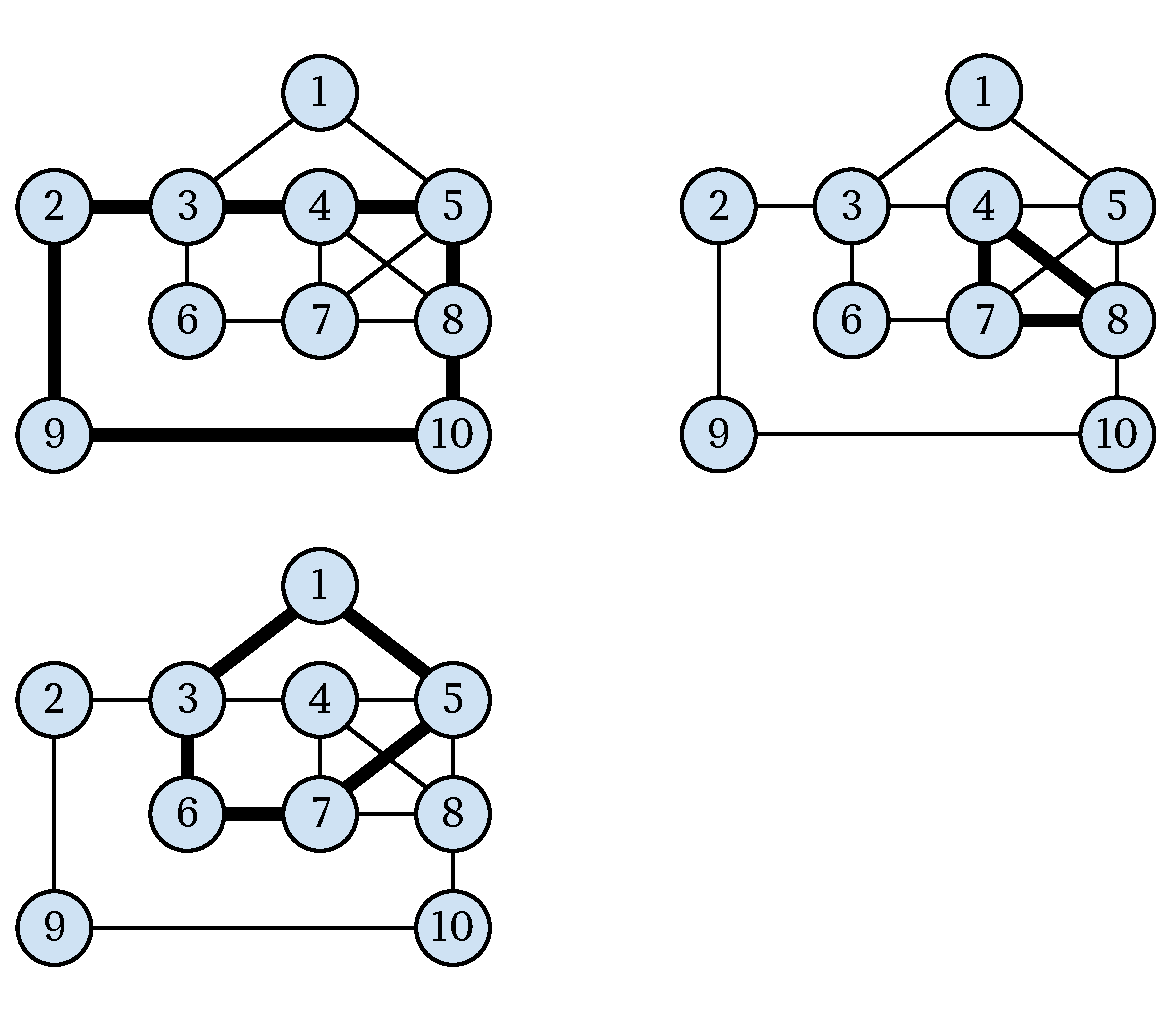
\includegraphics[width=7cm]{senior-example}

        Atkreipkite dėmesį, kad šiam pavyzdžiui egzistuoja keletas sprendinių,
        ir kai kuriuos iš jų sudaro tik du maršrutai.
    }

    \Scoring

    \begin{description}
        \item[Dalinė užduotis Nr. 1 (38 taškai):]
            $3 \le N \le 2\ 000$, $3 \le M \le 100\ 000$.
        \item[Dalinė užduotis Nr. 2 (17 taškų):]
            $3 \le N \le 100\ 000$, $3 \le M \le 100\ 000$.
        \item[Dalinė užduotis Nr. 3 (45 taškai):]
            $3 \le N \le 500\ 000$, $3 \le M \le 500\ 000$.
    \end{description}

    \Constraints

    \begin{description}
        \item[Laiko limitas:] 0,5 s.
        \item[Atminties limitas:] 256 MB.
    \end{description}

\end{document}
